\chapter[Rule-Based Performance-Bug Detection]{Rule-Based Performance-Bug Detection}
\label{chap:detec}

\section{Introduction}

%Automatic performance bug detection is important and challenging, as discussed
%in Section~\ref{sec:lessons}.
Rule-based detection approach is effective for discovering functional bugs
and security vulnerabilities \citep{chouasplos00,billpugh,PRMiner05,semanticpatch,fortify}. 
Many functional bugs can be identified by comparing against certain 
function-call sequences that have to be followed in a program 
for functional correctness and security.

We hypothesize that rule-based bug detection is useful for detecting performance 
bugs based on our characteristics study:

%\begin{itemize}

%\item 
\emph{Efficiency rules should exist.} Those inefficient function-call sequences 
studied in Section~\textcolor{red}{XX} could all become rules.
%  procedure boundary!!
For example, \Code{random()} should not be used by concurrent threads, and
\Code{doTransact()} in loops should be replaced by \Code{aggregateTransact()}.

%\item 
\emph{Efficiency rules can be easily collected from patches,} as 
%It is not difficult to collect rules from patches, because
most patches are small and follow regular fixing strategies 
(Section~\textcolor{red}{XX}).
%It will not be difficult to examine them and extract efficiency rules.
%TODO We did find 40 out of \allbugs bug patches containing rules.

\emph{Efficiency rules could be widely applicable,} as 
a misunderstanding of an API or workload could affect many places and
lead to many bugs, considering how bugs are introduced 
(Section~\textcolor{red}{XX}).

%\end{itemize}

This chapter will test our hypothesis and provide guidance for future work 
on combating performance bugs.
%\comment{
%Specifically, to test our hypothesis, we will answer the
%following questions:
%%How effective is it?
%%How applicable are efficiency rules;
%{\bf Q0:\ } Can rule-based approach discover previously unknown performance
%problems?
%{\bf Q1:\ } When fixing one performance bug, how many similar bugs did 
%developers miss? Will those bugs eventually get fixed?
%{\bf Q2:\ } After correcting a mistake, will developers make this
%mistake again?
%{\bf Q3:\ } Can we apply rules extracted from one application for
%another application?
%{\bf Q4:\ } Is violating rules rare compared with following the 
%rules?
%}

\section{Efficiency Rules in Patches}

\paragraph{Terminology} {\emph Efficiency rules}, or {\emph rules}, include two 
components: a {\emph transformation} and a {\emph condition} for applying the 
transformation. Once a code region satisfies the condition, 
the transformation can be applied to improve performance and preserve
functionality. 

We have manually checked all the 110 performance-bug patches.
50 out of these 110 patches contain efficiency rules, coming
from all five applications. 
The other 110 do not contain rules, because they
either target too specific program contexts or are too general to be useful
for rule-based bug detection.

\input chapter-detec/rule_tab.tex

Most of these 50 rules, according to the {\it lift} correlation metric,
are related to the {\it Uncoordinated Functions} root cause and the
{\it Change Call Sequence} fix strategy. 
The conditions for applying these rules are composed of
conditions on function-call sequences,
parameter/return variables,
and calling contexts, as shown in Table~\ref{tab:rule}.
For example, to apply the {\it Bookmark All} patch 
in Figure~\ref{fig:uncoord2} elsewhere, one 
needs to find places that call \Code{doTransact} inside a loop;
%\Code{::DeleteObject()} is followed by 
%\Code{::CreateRectRgn(,)} and the parameter of the former
%is the same variable that holds the return value of 
%the latter.
to apply the patch in Figure~\ref{fig:emp} elsewhere, one needs to ensure
that certain fields of the object pointed by the first parameter of 
\Code{apr\_stat} is not used afterward.
%\comment{
%For example, the patch of
%Apache48778 applies when \Code{DateFormat.getDateInstance()} is invoked by 
%only one thread or the number of its 
%invocation per thread outweighs the number of threads invoking it;
%the patch of MySQL38941 applies when multiple \Code{random()} could
%be called simultaneously by multiple threads. 
%For example, \Code{::DeleteObject( )} followed by \Code{::CreateRectRgn(,)}
%(Figure~\ref{fig:uncoord1}); \Code{doTransact()} is inside a loop,
%(Figure~\ref{fig:uncoord2}).
%}
There are also non-function rules, 
usually containing {\it Change Condition} transformation and other
miscellaneous algorithm improvements. 
%They do not have common templates.

%TODO: workload
%\comment{
%These rules are all useful for bug detection and fixing throughout the
%software. For 26 bugs in our study, developers applied similar
%patches at various locations in the code, when fixing them.
%%Note that these are {\bf not} copy-paste code regions.
%%Instead, they are code regions affected by the same understanding of particular
%%APIs or workload.
%Developers also complained about the manual effort involved in searching
%code regions that need similar patches in the discussion board.
%%After patching the bug shown in Figure~\ref{fig:emp}, 
%%a developer commented that
%%{\it `I believe there are other places that these occur'}.
%%Unfortunately, without tool support, the developers failed
%%to find all similar buggy code regions and left many unfixed.
%}

\section{Building Rule Checkers}

{\bf Selecting Statically Checkable Rules\ }
Some rules' applying conditions are statically checkable, such as function f1 
inside a loop; some are dynamically checkable, such as function f1 called by 
multiple threads at the same time; some are related to
workload, such as having many large input files. 
%First in first out :S.

We check three largest application suites in our study: Apache, MySQL, and Mozilla.
We find that 40 bug patches from them contain rules.
25 out of these 40 have applying conditions that are mostly statically
checkable. Therefore, we have built checkers based on these {{\bf 25} 
efficiency rules}.

{\bf Checker Implementation\ }
We build 25 checkers in total. 
14 of them are built using LLVM compiler infrastructure \citep{llvm} for 
rules from C/C++ applications. LLVM works well for C++ software that troubles 
many other static analysis infrastructure \citep{10yearlinux}. 
It also provides sufficient data type, data flow, and control 
flow analysis support for our checking. The other 11 checkers are 
written in Python for 11 rules from Java, JavaScript, and C\# applications.

%We build 25 checkers in total. 14 of them are built using LLVM compiler
%infrastructure \cite{llvm} for rules from
%C/C++ applications. 
%\comment{
%LLVM works well for C++ 
%software that troubles many other static analysis infrastructures
%\cite{10yearlinux}. It also
%provides sufficient data type, data flow, and control
%flow analysis support for our checking.}
%%The other 11 checkers are written in Python for 11 rules from 
%%Java, JavaScript, and C\# applications.

%%The checker implementation is straightforward, and mostly takes fewer
%%than 50 lines of code. 
%%Each checker goes through software bitcode, in case of LLVM checkers,
%%or source code, in case of Python checkers, and look for places that
%%satisfy the patch-applying condition.
%%Object type checking, control-flow analysis, intra-procedural data-flow
%%analysis, and loop identification are all used in our checkers.
%%Due to the space limit, we omit the implementation details of our
%%checkers.

The checker implementation is mostly straightforward. Each checker goes through 
software bitcode, in case of LLVM checkers, or source code, in case of Python 
checkers, looking for places that satisfy the patch-applying condition. We
briefly discuss how our checkers examine typical conditions for function rules in the following.

Checking call-sequence conditions, exemplified in Table~\ref{tab:rule}, involve mainly three tasks: 
(1) Differentiating functions with the same name but different classes; 
(2) Collecting loop information (loop-head, loop-exit conditions, 
loop-body boundaries, etc.); (3) Control flow analysis. 
%For example, 
%we need to check whether an invocation of f1 is post-dominated by 
%an invocation of f2. 
LLVM provides sufficient support for all these tasks. Checkers written in Python struggle from time to time.

Checking parameter/return conditions, exemplified in Table~\ref{tab:rule}, 
typically rely on data-flow analysis. In our current prototype, LLVM checkers 
conduct intra-procedural data-flow analysis. This analysis is scalable, 
but may lead to false positives and negatives. In practice, it works
well as shown by our experimental results. Our current Python checkers can 
extract parameters of particular function calls, but can only do preliminary data-flow analysis.

%An example of a LLVM checker found be found at the following URL: https://...


%TODO: rewrite to organize based on what type of analysis is needed?

\section{Rule-Checking Methodology}
\label{sec:detection_meth}

We conduct all the experiments on an 8-core Intel Xeon
machine running Linux version 2.6.18. 

We apply every checker to the following software: 

(1) The exact version of the software that the original patch was applied to, 
which is referred to as {\it original version}; 

(2) The latest version of 
the software that the original patch was applied to, which is referred to as 
{\it original software}; 

(3) The latest versions of 
software applications that are {\bf different} from the one that the original
patch was applied to, which is referred to as {\it different software}. 
This was applied to 13 checkers, whose rules are about {\it glibc} library
functions, Java library functions, and some general algorithm tricks. 
We will refer to this as {\it cross-application checking}.
For example, a C/C++ checker from MySQL will be applied to
Mozilla and Apache HTTPD for cross-application checking; a Java checker
from Apache TomCat server will be applied to the 65 other Java applications
in the Apache software suite\footnote{Development teams
behind different Apache applications are different}.

%Actually, the 13 checkers are applicable to {\it any} application that is 
%written in a particular programming language.

%\comment{
%Our checkers were applied to
%Mozilla (4.46 million lines of code, mainly C++), 
%MySQL (1.25 million lines of code, C/C++),
%Apache HTTPD (0.39 million lines of code, C), 
%and 66 Java applications from Apache suites (10.2 million lines of code).
%Note that developers behind different Apache applications are different.
%}

%As shown in Table~\ref{tab:category}, 
The checking results are categorized into three types: 
{\it PPPs}, {\it bad practices}, and {\it false positives}. 
As discussed in Section~\ref{sec:con2}, a PPP is an inefficient code region that
runs slower than its functionality-preserving alternate implied by
the efficiency rule. A bad practice is a region prone to becoming
inefficient in the future.
%Due to time constraints, we were unable to report all PPPs we found to
%developers.
We reported some PPPs to developers.
Among those reported, 14 PPPs detected by 6 different
checkers have been confirmed and fixed by the developers. 
Other reported PPPs are put on hold due to lack of
bug-triggering input information, which is unfortunately out of the 
scope of this work.

Finally, we have also changed each checker slightly to report
code regions that follow each efficiency rule. We refer to these regions as 
{\it good practices}, the opposite of PPPs. 

\section{Rule-Checking Results}
\label{sec:detection_results}

\input chapter-detec/detector_result_tab.tex

{\bf Overall Results\ }
%\subsubsection{Performance bugs}
As shown in Table~\ref{tab:detect_result}, 125 PPPs are found in the {\it original 
version} of software.
Programmers missed them and failed to fix them together with the original bugs.

%\underline{Answer to Q1, Q2}: 
113 previously unknown PPPs are found in the latest versions of the 
{\it original software}, including bugs inherited from the original version
and bugs newly introduced. Figure \ref{fig:newbug} shows an example. 

%\underline{Answer to Q3}: 
219 previously unknown PPPs are found in the latest versions of
{\it different software}. An example is shown in Figure \ref{fig:newbug}. 

14 PPPs in the latest versions of Apache, Mozilla, and MySQL
are already confirmed and fixed by developers based on our report.

These results confirm that performance bugs widely 
exist. Efficiency rules exist and are useful for finding
performance problems.

\begin{figure*}[t!]
\begin{center}
\begin{minipage}{3.3in}
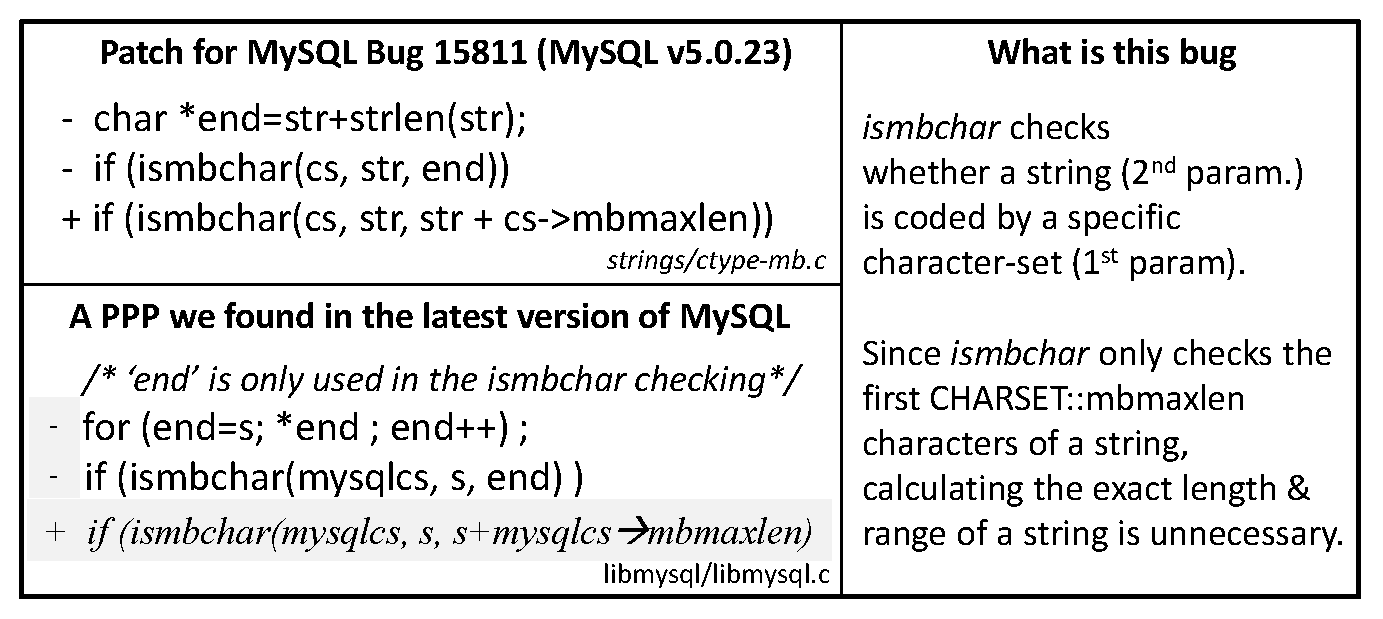
\includegraphics[height=1.42in]{figures/mysql15811.eps}
%\caption{\small PPP found in the same application}
%\label{fig:my15811}
\end{minipage}
\begin{minipage}{3in}
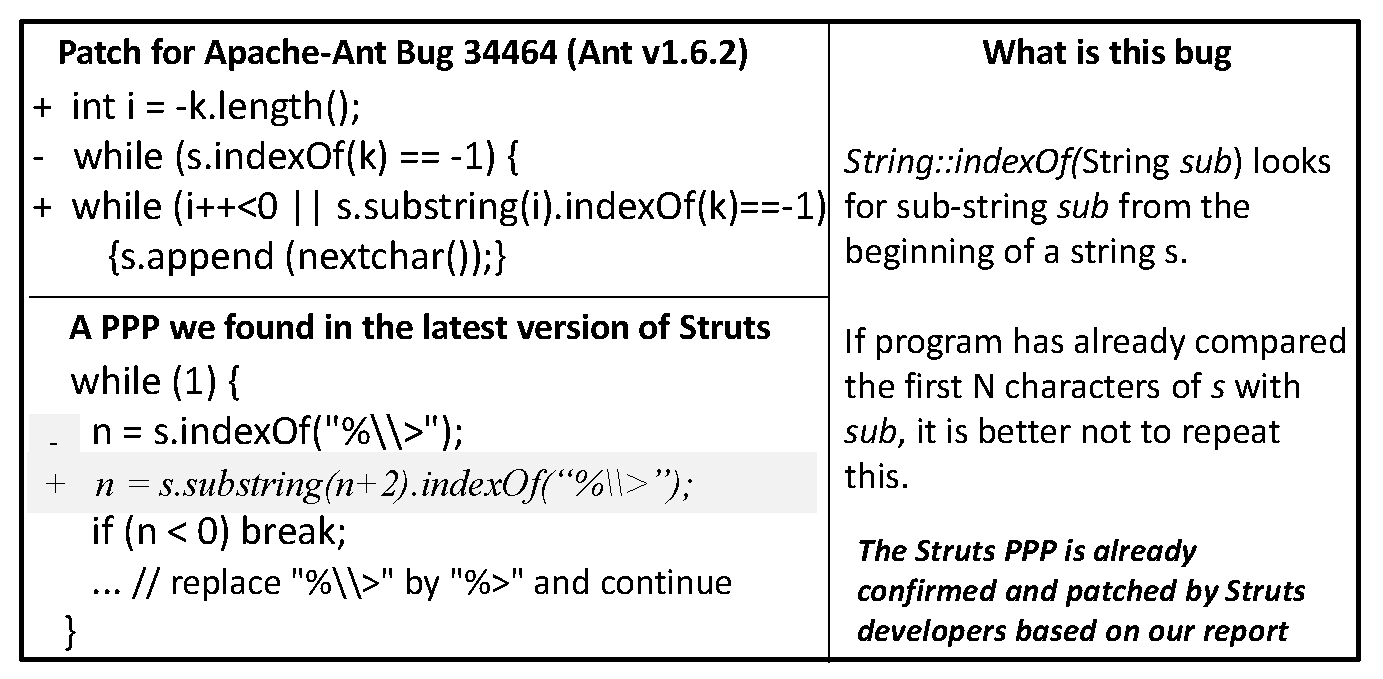
\includegraphics[height=1.42in]{figures/apache34464.eps}
%\caption{\small PPP found in a different application}
%\label{fig:ap34464}
\end{minipage}
\end{center}
\caption{PPPs we found in latest versions of {\it original} and {\it
different} software (the gray area shows how these two PPPs should be fixed)}
\label{fig:newbug}
\end{figure*}

{\bf PPPs In Original Versions\ }
17 out of 25 checkers found new PPPs, 125 in total, in the original versions
of the buggy software.
%that were missed by developers.

Some developers clearly tried to find all similar bugs when
fixing one bug, but did not succeed.
For example, in MySQL14637, after two buggy code regions were 
reported, developers found three more places that were similarly
inefficient and fixed them altogether. Unfortunately,
there were another 50 code regions that violated the same efficiency
rule and skipped developers' checking, as shown in 
Table~\ref{tab:result}. Similarly, MySQL developers found and fixed 3 places
that had the inefficiency pattern shown in Figure~\ref{fig:newbug},
but missed the other 15 places.

113 out of these 125 PPPs exist in different files or even different 
modules where the original bugs exist, which is probably why they were missed by
developers. These PPPs end up in several ways:
(1) 4 of them were fixed in later versions, which took 14--31 months;
(2) 20 eventually disappeared, because the
functions containing these PPPs were removed or re-implemented;
(3) 101 still exist in the latest versions of the software, wasting
computation resources 12--89 months after the original bugs were fixed.

\underline{Lesson\ } 
The above results show that developers do need support to systematically and 
automatically find similar performance bugs and fix them all at 
once.

{\bf PPPs In The Latest Versions\ }
2 of the 25 checkers are no longer applicable in the latest versions,
because the functions involved in these checkers
have been removed. The remaining 23 checkers are applied to
the latest versions of corresponding software and find
113 PPPs. Among them, 101 PPPs were
inherited from the original buggy versions.
The other 12 were introduced later. 

\underline{Lesson\ }
Developers cannot completely avoid the mistakes they made
and corrected before, which is understandable considering the large number of bugs in
software.
Specification systems and automated checkers can prevent developers 
from introducing old bugs into new code.
%programmers are still making the old mistakes. 

{\bf PPPs In Different Software Applications\ }
An exciting result is that 8 out of 13 cross-application checkers 
have successfully found previously unknown
PPPs in the latest versions of applications that are different from
where the rules came from.

Most of these checkers reflect common pitfalls in using
library functions. For example, Figure~\ref{fig:newbug} shows a pitfall
of using \Code{String::indexof()}. Apache-Ant developers made this
mistake, and we found Apache-Struts developers also made a similar mistake.

Apache32546 checker presents an interesting case. In the original 
bug report, developers from Apache-Slide recognized that
a small buffer size would severely hurt the performance of 
\Code{java.io.InputStream.read (byte buffer[])}
for reasonably large input
(e.g., larger than 50KB). Replacing their original
2KB buffer with a 200KB buffer achieved {\bf 80 times} throughput 
improvement in WebDav server. We first confirmed that this rule is
still valid. Our checker then found 135 places
in the latest versions of 36 software applications where similar mistakes were made.
These places use small buffers (1KB -- 4KB) to read images or data
files from disk or web, and are doomed to performance losses.

Some checkers reflect algorithm improvements and are also applicable to
many applications. For example, algorithm improvements for string operations 
proposed by MySQL developers (MySQL14637 and MySQL49491) also apply for
Mozilla and Apache HTTPD.


Cross-application checking also helps validate efficiency rules.
For example, by comparing how \Code{java.util.zip.Deflater.deflate()}
is used across applications, we found that Ant developers'
understanding of this API, reflected by their discussion, 
was wrong. They fixed Apache45396 by coincidence.

\underline{Lesson\ } 
The above results show that there exist general inefficiency patterns that
go beyond one application, just like that for functional
bugs \citep{billpugh}. 
Maintaining specifications and checkers for these general patterns can 
significantly save developers' effort, and allow them
to learn from other developers and other software. 
We can even discover performance bugs in a software where no
performance patch has ever been filed.
%TODO: software project, software application, confusing term.

\vspace{0.05in}
{\bf Bad Practices\ } 
Other than PPPs, some code regions identified by the 
checkers are categorized as bad practices.
For example, there are code regions very similar to
the MySQL PPP shown in Figure~\ref{fig:newbug}, except that the calculation of
\Code{end} is not completely useless as \Code{end} is used in places other than 
the invocation of \Code{ismbchar}.
Clearly this practice is more likely to cause performance problems
in the future than directly using
\Code{mysqlcs}$\rightarrow$\Code{mbmaxlen} as the parameter
for \Code{ismbchar} function.

\vspace{0.05in}
{\bf Good Practices\ }
Code regions that have well followed the efficiency rules are also identified
by slightly changed checkers.
For example, we found that in 13 places of various applications 
developers do use 
\Code{InputStream.read (byte buffer[])} in a performance efficient
way: \Code{buffer} has a configurable size or 
a large size that suits the workload (e.g., 64K in some Hadoop code).

\underline{Lesson\ } Violations to efficiency rules are not 
always rare comparing with good practices. 
Previous techniques that use statistical analysis to
infer functional rules \citep{PRMiner05,engler01bugs} 
may not work for efficiency rules.

{\bf False Positives\ }
Our PPP detection is accurate. 
On average, the false-positive-vs-PPP rate is 1:4.
The false positives mainly come from three sources.

First, Python checkers have no object-type information.
Therefore, some rules are applied to functions
with right function names but wrong classes
(e.g., Mozilla490742 and 
Apache32546). This is not a problem in LLVM checkers.

Second, some non-function rules are difficult to 
accurately express and check, which leads to false positives in
MySQL14637.

Third, accurately checking some efficiency rules requires run-time and/or 
workload information, which inevitably leads to false positives in
our static checkers. 
%This includes
%how many times a function is to be invoked, whether
%multiple threads could invoke a function concurrently, what is the typical
%length of an input, etc. 
False positives in Apache44408 and Apache48778 mostly belong to this 
category. These false positives can be largely eliminated by
run-time checkers.

{\bf Performance Results\ }
Our checkers are efficient. Each Python checker finishes
checking 10 million lines of code within 90 seconds.
Our LLVM checkers are mainly applied to 
MySQL, Mozilla Firefox, and Apache HTTPD.
It takes 4 -- 1270 seconds for one LLVM
checker to process one application.

We tried unit testing on PPPs.
The performance difference is significant. 
For example, for programs that read images and files using
\Code{InputStream.read}\Code{(byte buffer[])} with a 4KB-buffer parameter,
we can stably get 3 times throughput improvement through a 40K-buffer parameter.
When we feed the unit test with a 50MB file, which is a quite common image-file
workload these days,
the file operation time decreases from 0.87 second to 0.26 second,
a definitely perceivable difference.
As another example, the Struts code shown in Figure~\ref{fig:newbug}
is from a utility function used for processing JSP files. 
Our unit testing with a 15K JSP 
file shows that the simple patch can decrease latency by 0.1 second, 
a perceivable difference in interactive web applications.

Whole system testing turns out to be difficult, as suggested by our
characteristics study (Section~\ref{sec:char_exp}). 
No PPP detected by our checkers belongs to the always-active category. 
Future performance-oriented input-generation tools will significantly
help performance testing and identify truly severe PPPs. Execution frequency
information can also help future static performance-bug detectors to rank 
the severity of PPPs.

%TODO Our experience with developers. (1) If the patch is simple enough, 
%developers would do it.


\subsection{Discussions}

%TODO 1. original tone is too negative; should we put this earlier
%to lower the expectation?
{\bf Effectiveness of rule-based performance-bug detection\ }

{\it Effort saving\ } Rule-based detection not only identifies problems, but
also suggests alternative implementations with better efficiency.
These alternative implementations often
have small sizes and regular patterns,
as shown in Figure~\ref{fig:newbug}, 
making PPP validation and fixing easy.
It is also conceivable to enhance our checkers for automated PPP fixing. 

{\it Improving performance\ }
These PPPs showed 
significant performance improvement than their alternative implementations
in our unit testing. Without fixing these PPPs,
these unit-level performance losses could aggregate into intolerable
performance problems that are difficult to diagnose. 
This is especially significant considering that many performance bugs are
difficult to catch using other approaches.


{\it Maintaining code readability\ }
Like those 109 patches studied earlier, 
most PPPs detected by us can be fixed through changes to a few lines of code,
%and do not hurt code readability, 
as shown in Figure~\ref{fig:newbug}.
Even for the few complicated PPPs, wrapper-functions or 
macros can easily address the patch-readability issue.
%which is exactly what developers did in some of the patches we studied.

{\it Other usage\ }
Rules and checkers can serve as performance specifications for future 
software
development. They can aid in code maintenance when software evolves.
Developers can also save PPPs to an inefficiency list for future performance 
diagnosis.

Of course, this is only a starting point for rule-based performance-bug
detection. We expect our experience to motivate future work on 
automatically generating rules, checkers, or even patches.

%TODO you can automatically un-fix if you want
%TODO PPP xx is different from premature over-optimization.

\vspace{0.1in}
{\bf Can these problems be detected by other tools?\ }

{\it Copy-paste detectors\ } 
Most PPPs that we found are {\bf not} from copy-paste code regions
 and cannot be detected by text-matching tools
\citep{zhendong.oopsla10,CPMiner04}, as we can see in
Figure~\ref{fig:newbug}. Rule violations are not rare.
When developers misunderstand an API,
they tend to make mistakes whenever they use this API.
As a result, these mistakes usually go beyond
copy-paste code regions.

{\it Compiler optimization\ }
None of the bugs that provided the efficiency rules could be optimized
away by compilers used in Apache, MySQL, and Mozilla. Many PPPs 
involve library functions and algorithmic inefficiency, and
are almost impossible for a compiler to optimize
(Figure~\ref{fig:newbug}).
Even for the few cases where compiler optimization might help
(Figure~\ref{fig:emp}), 
the required inter-procedural and points-to analyses are not scalable
for real-world large software. 

{\it General rule-based bug detectors\ }
Ideas for detecting functional bugs can greatly benefit 
and inspire future research on performance bug detection.
However, many approaches cannot be directly applied.
Tools that automatically infer functional correctness rules 
\citep{engler01bugs,PRMiner05,livshits05dynamine} may not be suitable
for efficiency rules, because rule violations are not rare,
as shown in Table~\ref{tab:result}. In addition, many efficiency rules either
involve only one function or discourage multiple functions to be used together, 
making them unsuitable for tools that focus on function correlations. 


%TODO: gunami work infer complexity, ras bodik: 


%TODO: these are potential performance problems.
% how to use them: they might conflict with productivity, readability
% it could be better done by macro, wrapper, use for diagnosis


